\section{Inhalte hinzufügen}
\frame{
    \frametitle{Inhalte hinzufügen}
	Artikel sind dezentral im Zuständigkeitsbereich abzulegen, d.h. im passenden Ordner des Bereiches.
	Generell ist die zentrale Ablage von z.B. Nachrichten unter ``news'' zu vermeiden. 
    Artikeltypen:
    \begin{itemize}
        \item Ordner
        \item Bild
        \item Seite
        \item Datei
        \item Link
        \item Termin
        \item Nachricht
        \item Kollektion
    \end{itemize}
}
\frame{
    \frametitle{Inhalte hinzufügen}
    \begin{figure}[!h]
        \centering
    %\begin{wrapfigure}{r}{0.4\textwidth}
        %\vspace{-20pt}
        %\begin{center}
            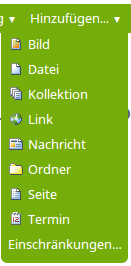
\includegraphics[width=0.33\textwidth]{../res/artikel-hinzufuegen.png}
        %\vspace{-20pt}
        %\end{center}
        \caption{Artikeltyp hinzuf\"ugen}
    %\end{wrapfigure}
    \end{figure}
}


\subsection{Kategorisierung}
\frame{
    \frametitle{Kategorisierung}
   \begin{itemize}
	\item Nicht persönliche Artikel jeden Typs sollten so umfangreich wie möglich kategorisiert werden. 
	\item Durch die Kategorisierung tauchen die Artikel in entsprechen Kollektionen auf
   \end{itemize}
   \begin{hinweis}
   \item Mehrere Stichworte müssen mit gedrückter \textit{Strg}-Taste ausgewählt werden.
   \end{hinweis}
    \begin{figure}[!h]
        \centering
        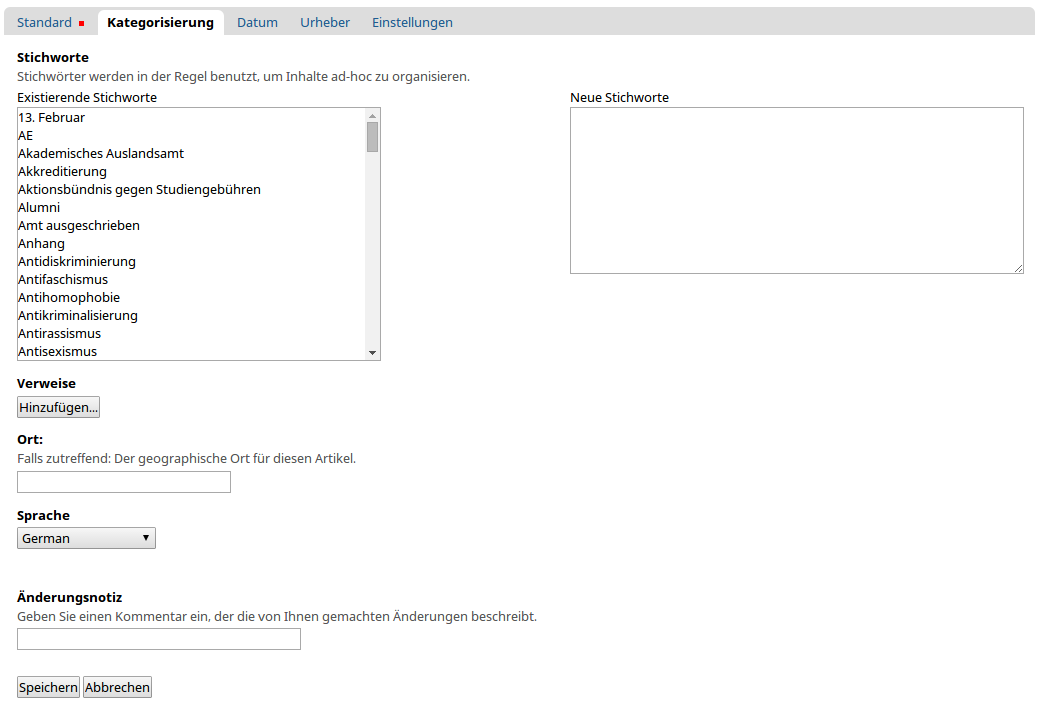
\includegraphics[width=0.66\textwidth]{../res/stura-kategorien.png}
    \end{figure}
}


\subsection{Artikeltypen}
\frame{
    \frametitle{Artikeltyp - Ordner}
    \begin{itemize}
        \item Angaben: Name, Titel, Beschreibung
        \item Startartikel: index\_html, index.html, index.htm, FrontPage
        \item Ansicht ändern
    \end{itemize}
    \begin{figure}[!h]
        \centering
        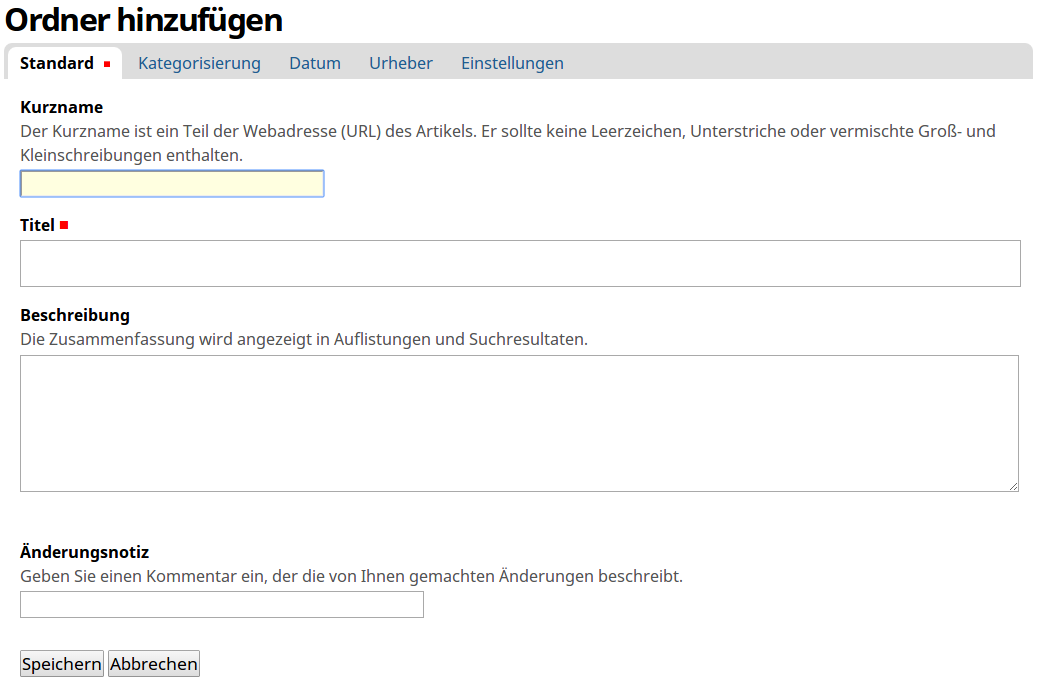
\includegraphics[width=0.75\textwidth]{../res/ordner-hinzufuegen.png}
    \end{figure}
}

\frame{
    \frametitle{Artikeltyp - Bild}
    Anschließend öffnet sich das folgende Formular:
    \begin{figure}[!h]
        \centering
        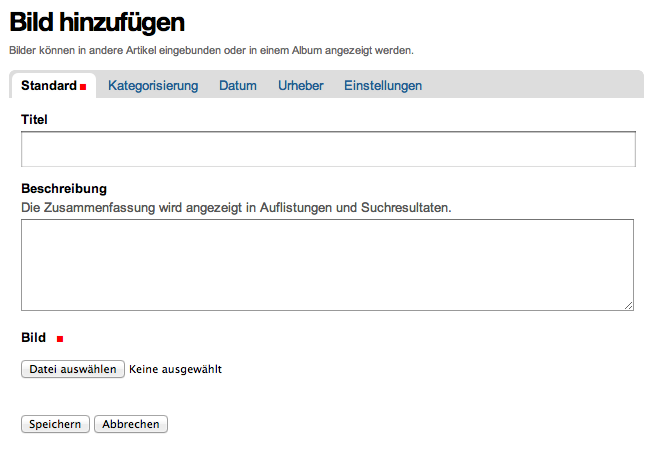
\includegraphics[width=\textwidth]{../res/bild-hinzufuegen_2.png}
    \end{figure}
}
\frame{
    \frametitle{Artikeltyp - Bild}
    \begin{description}
        \item[Titel] Aus dem Titel wird der Kurzname oder ID des Artikels gebildet.
 Wird kein Titel angegeben, behält das Bild üblicherweise seine ursprüngliche
 ID bei.

        \item[Beschreibung] Diese wird unter anderem bei der Anzeige von Suchergebnissen verwendet.

        \item[Bild] Klicken Sie auf *Datei auswählen* um auf Ihrem lokalen Computer eine Bilddatei zum Hochladen auszuwählen.
     Sie sollten die Bilder vor dem Auswählen für die Verwendung im Web vorbereiten.
     Eine kurze Anleitung hierzu finden Sie in der Präsentation *Erweiteres Wissen Website*
     unter dem Punkt``Bilder optimieren'' .

     Nach dem Hochladen wird Ihnen dann eine Vorschau des Bildes angezeigt.
        \item[Stichworte] Da Bilder nicht textuell erschlossen werden können, kommt den Stichworten eine besondere Bedeutung zu.
    \end{description}
}

\frame{
    \frametitle{Artikeltyp - Bild}
 \begin{tip}
     \item Eine Einführung zur Verschlagwortung von Bildern finden Sie unter
 `Verschlagwortungsstrategien
 \url{https://www.veit-schiele.de/profil/artikel/verschlagwortungsstrategien}`
 \end{tip}
}

\frame{
    \frametitle{Artikeltyp - Seite}
    \begin{itemize}
        \item Angaben: Name, Titel, Beschreibung, Eigenschaften
        \item Inhalte via Webbrowser eingebar
    \end{itemize}
    Dabei kann der Text in folgenden Formaten eingegeben werden:
    \begin{description}
        \item[HTML] ermöglicht Ihnen die direkte Eingabe von HTML;
        \item[Einfacher Text] ermöglicht Ihnen die einfache Eingabe von Text.
        \item[Markdown] ermöglicht Ihnen die direkte Eingabe mit Markdown-Syntax
    \end{description}

    Optional können Sie auch Textdateien auf den Server hochladen.
}

\frame{
    \frametitle{Artikeltyp - Datei}

	Dateiobjekte können Dateien enthalten, die heruntergeladen werden können.
	Hinzufügen:
	\begin{itemize}
	\item ``Durchsuchen\dots''-Taste klicken
	\item Verzeichnis durchsuchen, Datei auswählen
	\item ``Hochladen\dots''-Taste klicken
	\end{itemize}
	Die Bezeichnung, Beschreibung und Kategorisierung der Datei sind sehr relevant, da nur durch sie das einfache Auffinden der Datei gewährleistet werden kann.
    \begin{figure}
    %\begin{wrapfigure}{o}{\textwidth}
        %\vspace{-20pt}
        %\begin{center}
            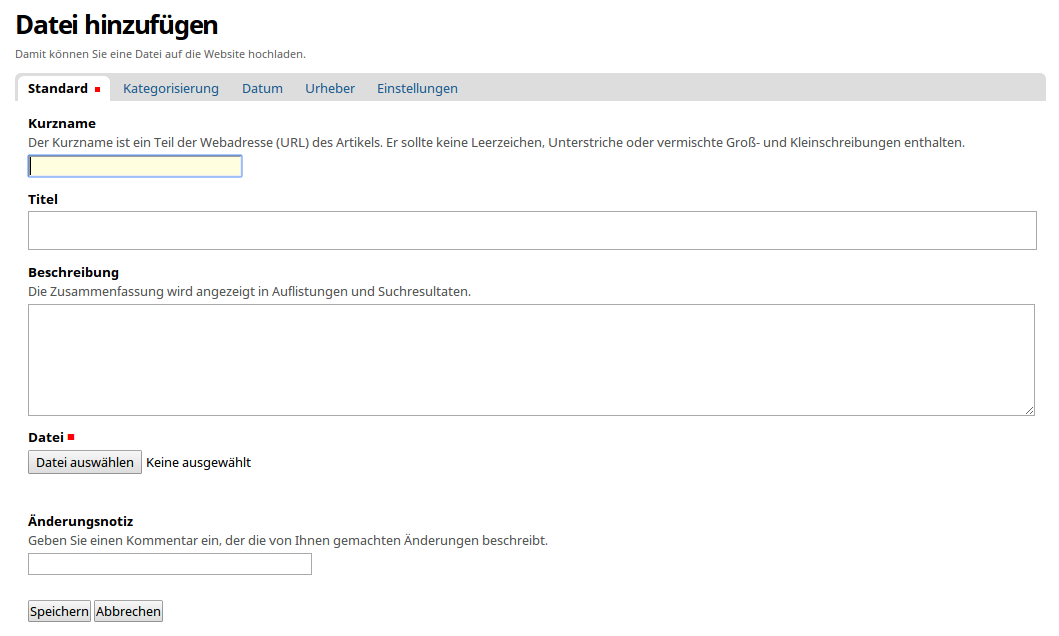
\includegraphics[width=0.5\textwidth]{../res/datei-hinzufuegen.png}
        %\vspace{-20pt}
        %\end{center}
        \caption{Datei hinzuf\"ugen}
    %\end{wrapfigure}
    \end{figure}
}

\frame{
    \frametitle{Artikeltyp - Link}
Links können als Schnellverweise gesetzt werden. 
So führt z.B. der Link \url{www.stura.htw-dresden.de/ese} für Externe direkt auf den Ordner der ESE. 
    Bitte beachten Sie bei der Angabe von externen Links die Angabe des Protokolls (z.B. ``http://'' für Webpages oder ``ftp://'' für Dateien).
}

\frame{
    \frametitle{Artikeltyp - Termin}
    Termine sind Objekte, die im Kalender eingetragen werden. Termine sollten im Ordner \textit{Termine} der ``zuständigsten'' Stelle, z.B Referat, Bereich oder Projekt eingetragen werden. Grundsätzlich sollten Termine von der Navigation ausgeschlossen werden. Dazu ist beim Artikel über Bearbeiten und Einstellungen ein Haken bei ``Von Navigation ausschließen'' zu setzen.

    \begin{itemize}
        \item Angabe: Name, Titel, Beschreibung
        \item weiter Ereignistypen, die auch als Schlagwörter verwendet werden
    \end{itemize}
    \begin{hinweis}
        \item Wollen Sie die Einträge in dieser Liste geändert haben, wenden Sie sich bitte an die Administration der Website.
    \end{hinweis}
}

\frame{
    \frametitle{Artikeltyp - Termin}
    \begin{description}
        \item[Terminanfang] Datum und Uhrzeit des Beginns; Sie können alternativ auch im nebenstehenden Kalender den Beginn auswählen.
        \item[Terminende] Datum und Uhrzeit können alternativ auch in nebenstehendem Kalender angegeben werden.
        \item[Terminort] Hier können Sie den Ort des Termins angeben.
        \item[Terminankündigung] Ankündigungstext für den Termin; alternativ können Sie auch eine Textdatei hochladen.
        \item[Teilnehmer] Teilnehmende des Termins.
        \item[Terminart] Die Art des Termins.
        \item[URL] Hier können Sie eine Web-Adresse angeben, die weitergehende Informationen über dieses Ereignis liefert.
        \item[Kontaktname] Kontaktperson oder -organisation für das Ereignis.
        \item[Kontaktadresse] Adresse, bei der Sie weitergehende Informationen zum Ereignis erhalten können.
        \item[Kontakt-E-Mail] E-Mail-Adresse für Nachfragen.
        \item[Kontakt-Telefon] Telefonnummer für Nachfragen und Reservierungen.
    \end{description}
}

\frame{
    \frametitle{Artikeltyp - Nachricht}
    Nachrichten sind Seiten  mit Titel, optionaler Beschreibung und Bild.

    Für Nachrichten lassen sich im Gegensatz zu Seiten noch je ein Bild mit Bildtitel angeben.
    \begin{figure}[!h]
        \centering
        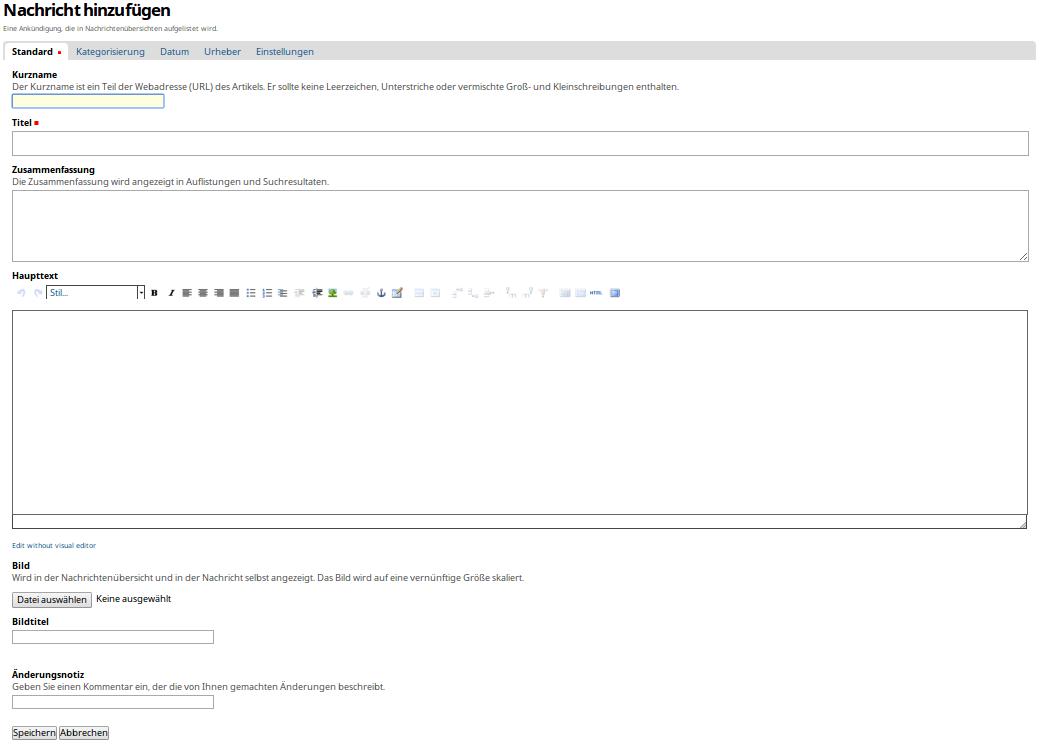
\includegraphics[width=0.75\textwidth]{../res/nachricht-hinzufuegen.png}
    \end{figure}
}

\frame{
    \frametitle{Artikeltyp - Kollektion}
    Kollektionen sind vorgefertigte Suchanfragen, die auch die Erschließung großer Datenbestände erlauben.

Kollektionen können üblicherweise nicht von allen Mitgliedern eines Portals hinzugefügt werden, sondern nur von denjenigen, die die Rollen *Website-Administrator* oder *Verwalter* innehaben. siehe: \url{www.stura.htw-dresden.de/stura/ref/verwaltung}
}
